\documentclass[a4paper,12pt]{article}

\usepackage{cmap}          % поиск в PDF
\usepackage{mathtext}         % русские буквы в формулах
\usepackage[T2A]{fontenc}      % кодировка
\usepackage[utf8]{inputenc}      % кодировка исходного текста
\usepackage[english,russian]{babel}  % локализация и переносы
\usepackage[left=2cm,right=2cm,top=2cm,bottom=2cm]{geometry}
\usepackage{amsfonts,amssymb,amsthm,mathtools} % AMS
\usepackage{amsmath}
\usepackage{icomma} % "Умная" запятая: $0,2$ --- число, $0, 2$
\usepackage{graphicx}
\usepackage{wrapfig} % картинка в тектсе
\usepackage{caption} % убирается номер у подписей caption*{}
\usepackage{csquotes} % цитаты
\usepackage{multirow} % для жестких таблиц
\usepackage{hhline}
\usepackage{indentfirst} % абзацный отступ после section
\usepackage{epigraph} % эпиграф
\usepackage{tikz}
\usepackage{pgfplots}
\usepackage[export]{adjustbox}
\usepackage{tabularx}
\usepackage{float}
\usepackage{longtable}

\title{\textbf{Измерение теплопроводности воздуха при атмосферном давлении. (2.2.3)}}
\author{Зайнуллин Амир Б05-206}

\begin{document}

\maketitle

\section{Аннотация}

\textbf{Цель работы:} измерить коэффициент теплопроводности воздуха при атмосферном давлении в зависимости от температуры. 

\textbf{В работе используются:} цилиндрическая колба с натянутой по оси нитью; термостат; вольтметр и амперметр (цифровые мультиметры); эталонное сопротивление; источник постоянного напряжения; реостат (или магазин сопротивлений).

\section{Теоретические сведения}

\textit{Теплопроводность} — это процесс передачи тепловой энергии от нагретых частей системы к холодным за счёт хаотического движения частиц среды. 

Перенос тепла описывается законом Фурье, утверждающим, что плотность потока энергии $\vec{q} ~ [\frac{Вт}{м^{2}}]$ (количество теплоты, переносимое   через единичную площадку в единицу времени) пропорциональна градиенту температуры:

\begin{equation*}
	\vec{q} = -\kappa \cdot \nabla T,
\end{equation*}

где $\kappa$ — \textit{коэффициент теплопроводности}.

\begin{equation*}
	\kappa \sim \lambda \bar{v} \cdot n c_v
\end{equation*}

где $\lambda$  — длина свободного пробега молекул газа, $\bar{v}$ — средняя скорость их теплового движения, n — концентрация газа.

В цилиндрически симметричной установке, в которой тепловой поток направлен к стенкам цилиндра от нити, полный поток тепла $Q = qS$ через каждую цилиндрическую поверхность радиуса $r$ должен в стационарном состоянии быть неизменен. Тогда

\begin{equation}
	Q = -2\pi rL\varkappa \frac{dT}{dr} = const,	
\end{equation}

откуда получаем формулу

\begin{equation}
	T_1 - T_2 = \frac{Q}{2\pi L\varkappa} \ln \frac{r_2}{r_1}.
\end{equation}

Здесь $r_1$ и $T_1$ -- радиус и температура нити, $r_2$ и $T_2$ -- радиус и температура цилиндра.

\begin{figure}[H]
    \centering
    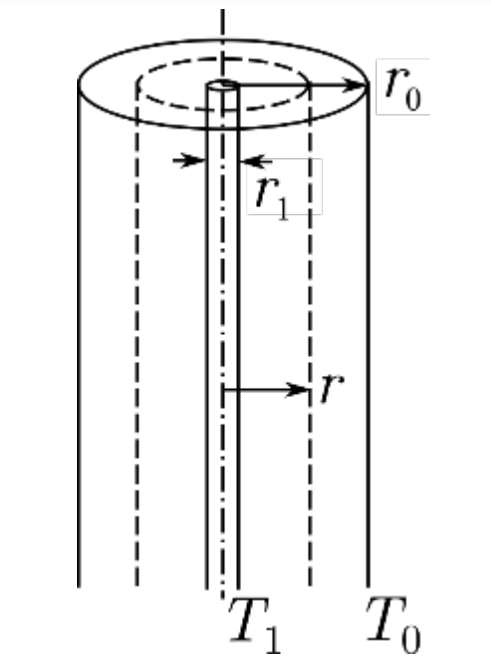
\includegraphics[width=0.25\textwidth]{first.png}
    \caption{Геометрия измерений}
\end{figure}

\section{Экспериментальная установка и методика измерений}

Схема установки представлена на рис. \ref{схема}. Полость трубки заполнена воздухом при атмосферном давлении, металлическая нить - источник тепла и датчик температуры.
\begin{figure}[H]
    \centering
    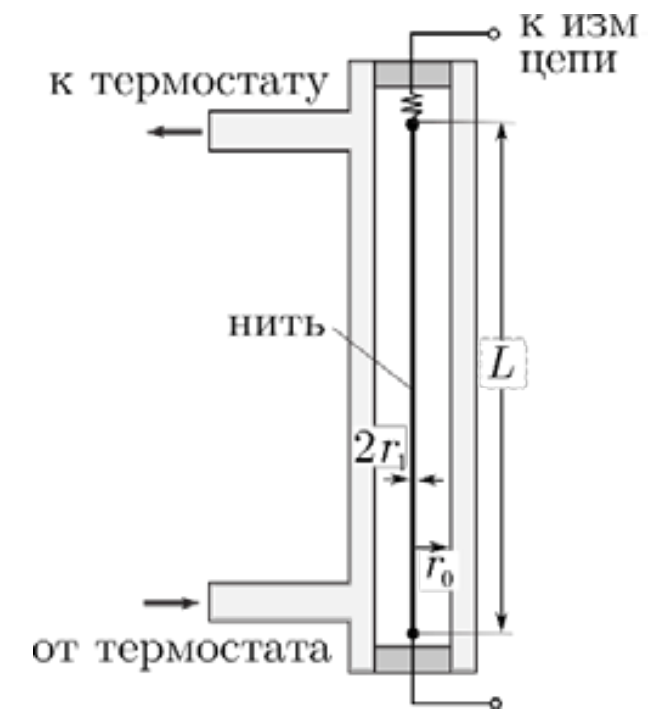
\includegraphics[width=0.3\textwidth]{схема.png}
\caption{Схема установки} \label{схема}
\end{figure}

\begin{figure}[H]
\centering
    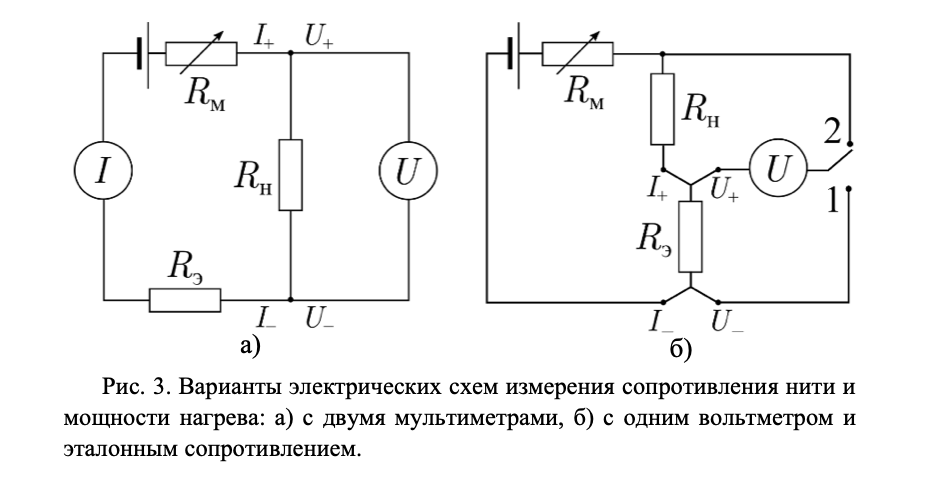
\includegraphics[width=0.65\textwidth]{электричество.png}
\end{figure}

Ток цепи регулируется с помощью магазина сопротивлений, включенного последовательно с источником напряжения.

Измерение нагрузочных кривых позволяет получить температурную зависимость сопротивления нити (при $Q \to 0$, $T\approx T_0$)

Для исследуемых температур:
\begin{equation}
R(t)=R_{273}\cdot(1+\alpha t)
\end{equation}
$\alpha=\frac{1}{R_{273}}\frac{dR}{dT}$  - температурный коэффициент сопротивления материала. По наклонам нагрузочных кривых можно получить значение коэффициента теплопроводности.

\subsection*{Методика измерений}
\begin{enumerate}
    \item Проведем предварительные расчеты параметров опыта. По формуле (2) оценим максимальную мощность нагрева. Далее определим максимальный ток и максимальное напряжение.
    \item Подготовим экспериментальную установку к работе 
    \item При фиксированной температуре термостата измерим зависимость сопротивления нити от подаваемой на нее мощности. Получим нагрузочную прямую.
    \item Измерения проведем для 9-10 значений тока. Ток следует наращивать монотонно, постепенно уменьшая сопротивление магазина сопротивлений. 
    \item Повторим 3-4 для 5-7 температур термостата. 
\end{enumerate}

\subsection*{Параметры установки}
\begin{enumerate}
    \item Материал нити - платина.
    \item $\ln \frac{r_2}{r_1} = 5$.
    \item Длина нити $L = 400 \pm 2$ мм.
    \item Сопротивление нити $R_н = 20$ Ом.
\end{enumerate}

\section{Результаты измерений и обработка данных}

По формулам посчитали максимальное напряжение, ток, мощность нагрева. $Q_{max} = 0,38$ Вт, $U_{max} = 2,8$ В, $I_{max} = 140$ мА. Далее получили нагрузочные кривые, данные записали в таблицы.


\begin{table}[H]
    \centering
    \begin{tabular}{|c|c|c|c|c|c|c|c|}
    \hline
        $U$, V & $\sigma_U,$ V & $I$, mA & $\sigma_I$, mA & $R_н$, Om & $\sigma_R$, Om & $Q$, mW & $\sigma_Q$, mW \\ \hline
        0,000792 & 0,000004 & 0,0382 & 0,0002 & 20,7330 & 0,2116 & 0,000030 & 0,0000 \\ \hline
        0,20997 & 0,00002 & 10,2070 & 0,0053 & 20,57118 & 0,0122 & 2,1432 & 0,0024 \\ \hline
        0,41653 & 0,00002 & 20,2045 & 0,0103 & 20,61570 & 0,0117 & 8,4158 & 0,0091 \\ \hline
        0,62180 & 0,00003 & 30,0680 & 0,0152 & 20,67979 & 0,0115 & 18,6963 & 0,0199 \\ \hline
        0,83262 & 0,00008 & 40,0848 & 0,0202 & 20,77146 & 0,0125 & 33,3754 & 0,0369 \\ \hline
        1,04845 & 0,00009 & 50,2020 & 0,0253 & 20,88463 & 0,0123 & 52,6343 & 0,0574 \\ \hline
        1,27640 & 0,00009 & 60,6842 & 0,0305 & 21,03348 & 0,0121 & 77,4573 & 0,0837 \\ \hline
        1,48280 & 0,00010 & 69,9936 & 0,0352 & 21,18479 & 0,0121 & 103,7865 & 0,1115 \\ \hline
        1,71210 & 0,00011 & 80,1020 & 0,0403 & 21,37400 & 0,0121 & 137,1426 & 0,1466 \\ \hline
        1,94640 & 0,00012 & 90,1615 & 0,0453 & 21,58793 & 0,0122 & 175,4903 & 0,1869 \\ \hline
    \end{tabular}
    \caption{Результаты измерений при $T = 25$ $^\circ$C}
\end{table}

\begin{table}[H]
    \centering
    \begin{tabular}{|c|c|c|c|c|c|c|c|}
    \hline
        $U$, V & $\sigma_U,$ V & $I$, mA & $\sigma_I$, mA & $R_н$, Om & $\sigma_R$, Om & $Q$, mW & $\sigma_Q$, mW \\ \hline
        0,000798 & 0,000004 & 0,0382 & 0,0002 & 20,89005 & 0,2125 & 0,000030 & 0,0000 \\ \hline
        0,20597 & 0,00002 & 9,9372 & 0,0052 & 20,72717 & 0,0123 & 2,0468 & 0,0023 \\ \hline
        0,41660 & 0,00002 & 20,0690 & 0,0102 & 20,75838 & 0,0118 & 8,3607 & 0,0090 \\ \hline
        0,62512 & 0,00003 & 30,0348 & 0,0152 & 20,81319 & 0,0116 & 18,7754 & 0,0200 \\ \hline
        0,83635 & 0,00008 & 40,0330 & 0,0202 & 20,89151 & 0,0125 & 33,4816 & 0,0370 \\ \hline
        1,05245 & 0,00009 & 50,1295 & 0,0253 & 20,99462 & 0,0123 & 52,7588 & 0,0575 \\ \hline
        1,26880 & 0,00009 & 60,0780 & 0,0302 & 21,11921 & 0,0122 & 76,2270 & 0,0824 \\ \hline
        1,48960 & 0,00010 & 70,0395 & 0,0352 & 21,26800 & 0,0122 & 104,3308 & 0,1121 \\ \hline
        1,71550 & 0,00011 & 80,0030 & 0,0402 & 21,44295 & 0,0122 & 137,2451 & 0,1467 \\ \hline
        1,94930 & 0,00012 & 90,0600 & 0,0452 & 21,64446 & 0,0122 & 175,5540 & 0,1870 \\ \hline
    \end{tabular}
    \caption{Результаты измерений при $T = 40$ $^\circ$C}
\end{table}

\begin{table}[H]
    \centering
    \begin{tabular}{|c|c|c|c|c|c|c|c|}
    \hline
        $U$, V & $\sigma_U,$ V & $I$, mA & $\sigma_I$, mA & $R_н$, Om & $\sigma_R$, Om & $Q$, mW & $\sigma_Q$, mW \\ \hline
        0,000794 & 0,000004 & 0,0381 & 0,0002 & 20,83990 & 0,2127 & 0,000030 & 0,0000 \\ \hline
        0,20760 & 0,00002 & 10,0230 & 0,0052 & 20,71236 & 0,0123 & 2,0808 & 0,0023 \\ \hline
        0,41629 & 0,00002 & 20,0680 & 0,0102 & 20,74397 & 0,0118 & 8,3541 & 0,0090 \\ \hline
        0,62472 & 0,00003 & 30,0348 & 0,0152 & 20,79987 & 0,0116 & 18,7633 & 0,0200 \\ \hline
        0,83588 & 0,00008 & 40,0345 & 0,0202 & 20,87899 & 0,0125 & 33,4640 & 0,0370 \\ \hline
        1,05190 & 0,00009 & 50,1329 & 0,0253 & 20,98223 & 0,0123 & 52,7348 & 0,0575 \\ \hline
        1,27970 & 0,00009 & 60,6060 & 0,0305 & 21,11507 & 0,0122 & 77,5575 & 0,0838 \\ \hline
        1,48900 & 0,00010 & 70,0494 & 0,0352 & 21,25643 & 0,0121 & 104,3036 & 0,1121 \\ \hline
        1,71490 & 0,00011 & 80,0178 & 0,0402 & 21,43148 & 0,0121 & 137,2225 & 0,1467 \\ \hline
        1,94860 & 0,00012 & 90,0770 & 0,0452 & 21,63260 & 0,0122 & 175,5240 & 0,1870 \\ \hline
    \end{tabular}
    \caption{Результаты измерений при $T = 55$ $^\circ$C}
\end{table}

\begin{table}[!ht]
    \centering
    \begin{tabular}{|c|c|c|c|c|c|c|c|}
    \hline
        $U$, V & $\sigma_U,$ V & $I$, mA & $\sigma_I$, mA & $R_н$, Om & $\sigma_R$, Om & $Q$, mW & $\sigma_Q$, mW \\ \hline
        0,000794 & 0,000004 & 0,0380 & 0,0002 & 20,89474 & 0,2136 & 0,000030 & 0,0000 \\ \hline
        0,20755 & 0,00002 & 10,0238 & 0,0052 & 20,70572 & 0,0123 & 2,0804 & 0,0023 \\ \hline
        0,41621 & 0,00002 & 20,0697 & 0,0102 & 20,73823 & 0,0118 & 8,3532 & 0,0090 \\ \hline
        0,62458 & 0,00003 & 30,0374 & 0,0152 & 20,79341 & 0,0116 & 18,7608 & 0,0200 \\ \hline
        0,83570 & 0,00008 & 40,0384 & 0,0202 & 20,87246 & 0,0125 & 33,4601 & 0,0370 \\ \hline
        1,05010 & 0,00009 & 50,0644 & 0,0252 & 20,97498 & 0,0123 & 52,5726 & 0,0573 \\ \hline
        1,26800 & 0,00009 & 60,0930 & 0,0302 & 21,10063 & 0,0122 & 76,1979 & 0,0824 \\ \hline
        1,48880 & 0,00010 & 70,0608 & 0,0352 & 21,25011 & 0,0121 & 104,3065 & 0,1121 \\ \hline
        1,71460 & 0,00011 & 80,0311 & 0,0402 & 21,42417 & 0,0121 & 137,2213 & 0,1467 \\ \hline
        1,95370 & 0,00012 & 90,3185 & 0,0454 & 21,63123 & 0,0122 & 176,4553 & 0,1879 \\ \hline
    \end{tabular}
    \caption{Результаты измерений при $T = 70$ $^\circ$C}
\end{table}

Убедимся, что графики линейны. Проведем прямые по МНК и найдем их точку пересечения с осью ординат, и также коэффициент наклона прямых. Данные запишем в таблицу.

\begin{figure}[H]
    \begin{minipage}[h]{0.49\linewidth}
    \center{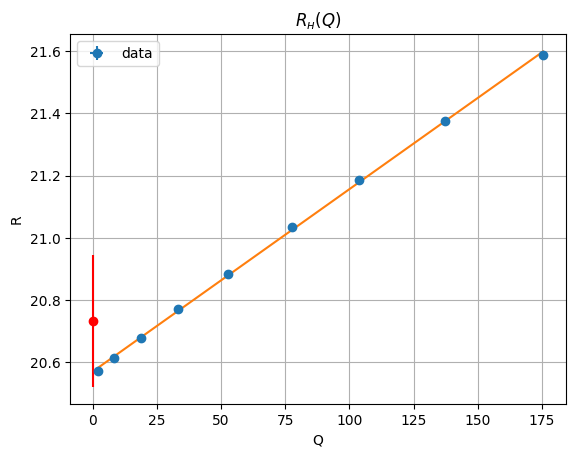
\includegraphics[width=1\linewidth]{25.png}}
    \caption{график для $T = $ 25 $^\circ$C}
    \end{minipage}
    \hfill
    \begin{minipage}[h]{0.49\linewidth}
    \center{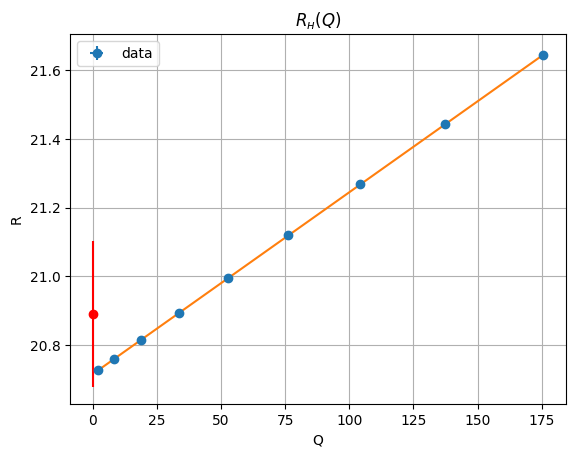
\includegraphics[width=1\linewidth]{40.png}}
    \caption{график для $T = $ 40 $^\circ$C}
    \end{minipage}
\end{figure}

\begin{figure}[H]
    \begin{minipage}[h]{0.49\linewidth}
    \center{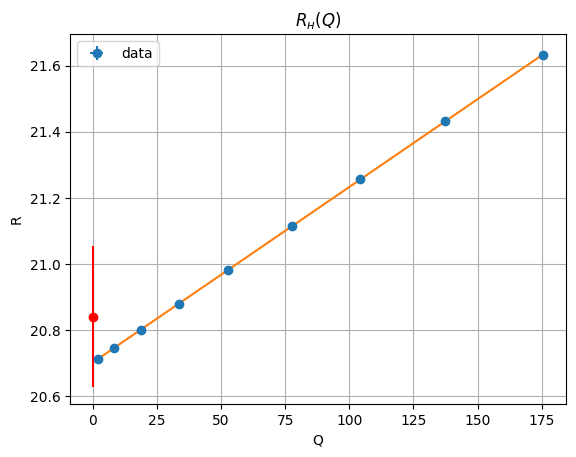
\includegraphics[width=1\linewidth]{55.png}}
    \caption{график для $T = $ 55 $^\circ$C}
    \end{minipage}
    \hfill
    \begin{minipage}[h]{0.49\linewidth}
    \center{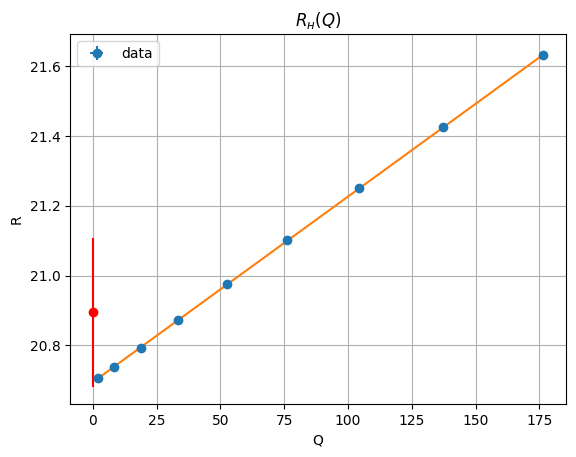
\includegraphics[width=1\linewidth]{70.png}}
    \caption{график для $T = $ 70 $^\circ$C}
    \end{minipage}
\end{figure}

\begin{table}[H]
    \centering
    \begin{tabular}{|c|c|c|c|c|}
    \hline
        $T$ $^\circ$C & $\dfrac{dR}{dQ}$, $\dfrac{Ом}{мВт}$ & $\sigma$ , $\dfrac{Ом}{мВт}$ & $R_0$, Ом & $\sigma_{R_0}$, Ом \\ \hline
        25 & 0,00586 & 0,00005 & 20,55 & 0,00005 \\ \hline
        40 & 0,00530 & 0,00001 & 20,88 & 0,00048 \\ \hline
        55 & 0,00532 & 0,00001 & 21,21 & 0,00064 \\ \hline
        70 & 0,00532 & 0,00001 & 21,54 & 0,00048 \\ \hline
    \end{tabular}
    \caption{Полученные результаты}
\end{table}

По данной таблице построим график сопротивления нити от ее температуры R(T). Построим прямую по МНК и определим ее наклон и также $R_{273}$. Данные запишем в таблицу.

\begin{figure}[H]
    \centering
    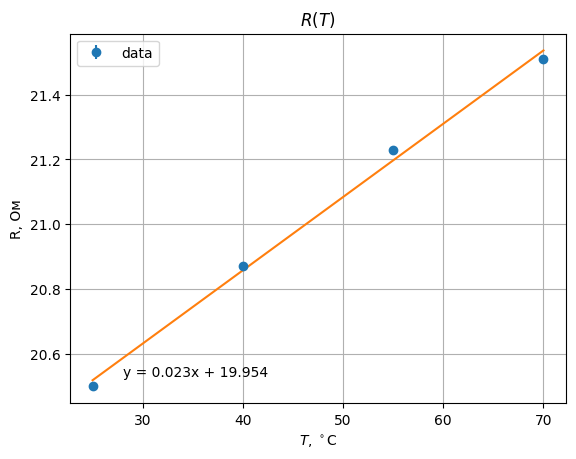
\includegraphics[width=0.7\textwidth]{R(T)_new.png}
\caption{График R от T}
\end{figure}

\begin{table}[H]
    \centering
    \begin{tabular}{|c|c|c|c|c|}
    \hline
        $\dfrac{dR}{dT}$, , $\dfrac{Ом}{К}$   & $\sigma$, $\dfrac{Ом}{К}$  & $R_{273}$, Ом  & $\alpha$, $\frac{1}{K}$ & $\sigma_{\alpha}$,  $\frac{1}{K}$ \\ \hline
        0,023 & 0,001 & 19,95 $\pm$ 0,05 & 0,00100 & 0,00005 \\ \hline
    \end{tabular}
    \caption{Результаты зависимости R(T)}
\end{table}

Найдем коэффициент теплопроводности воздуха для каждой температуры, используя прошлые полученные данные. 

\begin{table}[H]
    \centering
    \begin{tabular}{|c|c|c|c|c|c|c|}
    \hline
        $T$ К & $\dfrac{dR}{dQ}$, $\dfrac{Ом}{мВт}$ & $\sigma$ , $\dfrac{Ом}{мВт}$ & $\dfrac{dQ}{d(\Delta T)}$, $\dfrac{К}{мВт}$& $\sigma$, $\dfrac{К}{мВт}$& $\kappa$ $\dfrac{мВт}{м \cdot К}$ & $ \sigma_{\kappa}$, $\dfrac{мВт}{м \cdot К}$ \\ \hline
        298 & 0,00586 & 0,00005 & 3,9249 & 0,2041 & 0,4080 & 0,0211 \\ \hline
        313 & 0,00500 & 0,00001 & 4,6000 & 0,2092 & 0,4101 & 0,0189 \\ \hline
        328 & 0,00490 & 0,00001 & 4,6939 & 0,2137 & 0,4313 & 0,0193 \\ \hline
        343 & 0,00480 & 0,00001 & 4,7917 & 0,2183 & 0,4410 & 0,0198 \\ \hline
    \end{tabular}
    \caption{коэффициенты теплопроводности воздуха}
\end{table}

Построим график $\kappa(T)$. 

\begin{figure}[H]
    \centering
    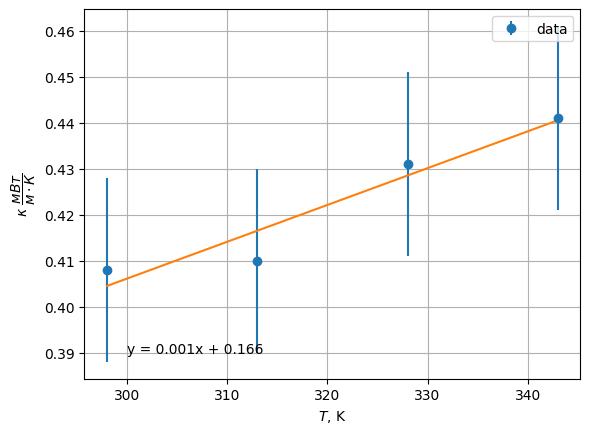
\includegraphics[width=0.7\textwidth]{kappa_new.png}
\caption{График $\kappa$ от T}
\end{figure}

\begin{table}[!ht]
    \centering
    \begin{tabular}{|c|c|}
    \hline
        $\ln (T)$ & $\ln(\kappa)$ \\ \hline
        5,6971 & -0,9011 \\ \hline
        5,7462 & -0,8766 \\ \hline
        5,7930 & -0,8555 \\ \hline
        5,8377 & -0,8340 \\ \hline
    \end{tabular}
\end{table}

\begin{figure}[H]
    \centering
    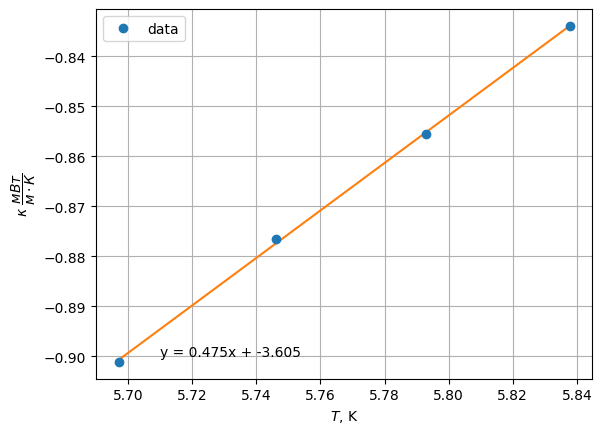
\includegraphics[width=0.7\textwidth]{ln_new.png}
\caption{График в логарифмическом масштабе}
\end{figure}

По МНК получили коэффициент $\beta = 0,475$. 

\section{Выводы}

\begin{enumerate}
    \item В ходе работы была экспериментально определена теплопроводность воздуха при различных температурах и обнаружена линейная зависимость этих величин. 
    \item Для каждой температура была построена нагрузочная кривая, которая является линейной зависимостью. Она была экстраполирована до пересечения с осью ординат, чтобы найти $R_0$. Первая точка (красного цвета) не ложилась на прямую потому что возможно из за маленького напряжения и тока, и, вследствие, мощности. Возможно установка еще не пришла в стационарное состояние. Также видно что у этой точки большая погрешность, и построенная прямая проходила через нее. 
    \item Далее был построен график зависимости $R(T)$. Точки были промоделированы по значению $R_{273} = 20$ Ом. Посчитан коэффициент наклона графика. С помощью его посчитали коэффициент теплопроводности воздуха для различных температур.
    \item Построили график по полученным значениям. Мы получили совсем другое значение $\kappa$, отличающееся от табличных 0,022 Вт/(м·K). Возможно это произошло из за неправильных точек графиков R(Q). из за этого могли получиться неверные коэффициенты $\dfrac{dQ}{dR}$. Возможно теоретическая модель которая используется в лабораторной работе выполняется не идеально. 
    \item Коэффициент $\beta$ сошелся с тем, что ожидается из теории (0,5). 
\end{enumerate}





\end{document}